\documentclass[12pt,a4paper]{report}

% ── Packages ────────────────────────────────────────────────────────────────
\usepackage[top=1in,bottom=1in,left=1.5in,right=1in,headheight=15pt]{geometry}
\usepackage{graphicx}
\usepackage[hidelinks]{hyperref}
\usepackage{setspace}
\usepackage{titlesec}
\usepackage{fancyhdr}
\usepackage{booktabs}
\usepackage{array}
\usepackage{mathptmx}
\usepackage{microtype}
\usepackage{enumitem}
\usepackage{tikz}
\usetikzlibrary{shapes.geometric,arrows.meta,positioning,fit}
\usepackage{caption}
\usepackage{url}
\usepackage{amsmath}
\usepackage{amssymb}

% ── Spacing ─────────────────────────────────────────────────────────────────
\onehalfspacing
\setlength{\parindent}{0pt}
\setlength{\parskip}{7pt}

% ── Chapter / section headings ──────────────────────────────────────────────
\titleformat{\chapter}[display]
  {\normalfont\Large\bfseries\centering}
  {Chapter \thechapter}{4pt}{\Large\centering}
\titlespacing*{\chapter}{0pt}{-10pt}{18pt}

\titleformat{\section}{\normalfont\large\bfseries}{\thesection}{1em}{}
\titleformat{\subsection}{\normalfont\normalsize\bfseries}{\thesubsection}{1em}{}
\titleformat{\subsubsection}{\normalfont\normalsize\bfseries}{\thesubsubsection}{1em}{}

% ── Headers / footers ───────────────────────────────────────────────────────
\pagestyle{fancy}
\fancyhf{}
\fancyhead[R]{\small\textit{NutriAI: Mid-Term Defense Report}}
\fancyfoot[C]{\thepage}
\renewcommand{\headrulewidth}{0.4pt}
\fancypagestyle{plain}{\fancyhf{}\fancyfoot[C]{\thepage}\renewcommand{\headrulewidth}{0pt}}

% ── TikZ styles shared by diagrams ──────────────────────────────────────────
\tikzset{
  startstop/.style={ellipse,draw,fill=gray!20,minimum width=3.0cm,
                    minimum height=0.75cm,align=center,font=\small},
  process/.style  ={rectangle,draw,fill=blue!10,minimum width=4.5cm,
                    minimum height=0.75cm,align=center,font=\small},
  decision/.style ={diamond,draw,fill=orange!20,minimum width=2.8cm,
                    minimum height=0.9cm,align=center,aspect=2.2,font=\small},
  filter/.style   ={rectangle,draw,fill=red!10,minimum width=4.5cm,
                    minimum height=0.75cm,align=center,font=\small},
  mlnode/.style   ={rectangle,draw,fill=green!15,minimum width=4.5cm,
                    minimum height=0.75cm,align=center,font=\small},
  arr/.style      ={-{Stealth[length=6pt]},thick}
}

% ════════════════════════════════════════════════════════════════════════════
\begin{document}

% ── Title Page ──────────────────────────────────────────────────────────────
\begin{titlepage}
\centering
\vspace*{0.3cm}
{\large\bfseries PURBANCHAL UNIVERSITY}\\[0.15cm]
{\normalsize\bfseries DEPARTMENT OF COMPUTER ENGINEERING}\\[0.1cm]
{\normalsize\bfseries KHWOPA ENGINEERING COLLEGE}\\[0.1cm]
{\normalsize LIBALI-08, BHAKTAPUR}\\[0.9cm]
\rule{\textwidth}{1.2pt}\\[0.3cm]
{\large\bfseries A MID-TERM PROJECT DEFENSE REPORT}\\[0.2cm]
{\normalsize ON}\\[0.45cm]
{\Large\bfseries NutriAI: AI-Powered Personalized Nutrition Recommendation and Calorie Tracking System}\\[0.3cm]
\rule{\textwidth}{1.2pt}\\[0.6cm]

{\normalsize Submitted in partial fulfillment of the requirements for the degree of}\\[0.3cm]
{\normalsize\bfseries Bachelor of Engineering in Computer Engineering (Seventh Semester)}\\[1.2cm]

{\large\bfseries Submitted by}\\[0.4cm]
{\normalsize
\begin{tabular}{ll}
\textbf{Dristi Shrestha}  & (790312) --- Frontend Lead \\[0.18cm]
\textbf{Prashant Ghimire} & (790328) --- Backend Lead \\[0.18cm]
\textbf{Romina Koju}      & (790332) --- ML Engineer \\[0.18cm]
\textbf{Shrijan Sainju}   & (790338) --- System Integration \& GenAI
\end{tabular}}\\[1.2cm]

{\normalsize\bfseries Department of Computer Engineering}\\
{\normalsize Khwopa Engineering College}\\
{\normalsize Libali-08, Bhaktapur, Nepal}\\[0.3cm]
{\normalsize September 2026}
\end{titlepage}

% ── Acknowledgement ─────────────────────────────────────────────────────────
\chapter*{Acknowledgement}
\addcontentsline{toc}{chapter}{Acknowledgement}
\thispagestyle{plain}

We express our sincere gratitude to Purbanchal University and the Department of Computer Engineering, Khwopa Engineering College, for providing the academic platform, computational infrastructure, and scholarly environment required to conduct this seventh-semester engineering project.

We extend our deepest appreciation to our project supervisor and esteemed faculty members for their continuous technical mentorship, constructive critiques, and insightful guidance throughout our architecture evaluations, data engineering pipelines, and mid-term assessments. Their feedback was instrumental in refining our machine learning formulation, hard safety filtering mechanisms, and conversational AI integration.

We also recognize the dedicated teamwork, technical contributions, and collaborative effort of all four team members: Dristi Shrestha (Frontend Lead), Prashant Ghimire (Backend Lead), Romina Koju (ML Engineer), and Shrijan Sainju (System Integration \& GenAI). Each member's commitment has been indispensable to the successful realization of this mid-term milestone.

Finally, we express our heartfelt appreciation to our families and colleagues for their constant encouragement, patience, and moral support throughout the course of this work.

\vspace{0.8cm}
\noindent With Regards,

\vspace{0.5cm}
\noindent Dristi Shrestha \hfill (790312)\\[0.1cm]
\noindent Prashant Ghimire \hfill (790328)\\[0.1cm]
\noindent Romina Koju \hfill (790332)\\[0.1cm]
\noindent Shrijan Sainju \hfill (790338)

\newpage

% ── Abstract ────────────────────────────────────────────────────────────────
\chapter*{Abstract}
\addcontentsline{toc}{chapter}{Abstract}
\thispagestyle{plain}

This mid-term defense report presents the design, mathematical formulation, and full-stack implementation progress of \textbf{NutriAI}, an AI-Powered Personalized Nutrition Recommendation and Calorie Tracking System tailored for Nepali dietary patterns. Conventional dietary tracking applications depend almost exclusively on Western nutritional databases, completely omitting traditional South Asian and Nepali preparations. Furthermore, existing systems either employ arbitrary heuristic scores or attempt to predict caloric content directly through statistical machine learning, leading to mathematical inaccuracies and a failure to enforce clinical safety constraints.

To address these limitations, NutriAI introduces a multi-tier \textbf{Separation of Concerns} architecture that decouples deterministic nutritional tracking from machine learning-based personalization. The core technical contributions achieved by the mid-term phase include:
\begin{enumerate}[leftmargin=*]
  \item \textbf{NepaliNutriDB Dataset:} Compilation and verification of an authoritative 129-food database of authentic Nepali staples and regional cuisine, with complete nutritional attributes (calories, protein, carbohydrates, fats, fiber, sugar, sodium) and bilingual Devanagari nomenclature, benchmarked against FAO Nepal (2012), NARC, and USDA FoodData Central.
  \item \textbf{Deterministic Nutrition Engine:} Implementation of the scientific Mifflin-St Jeor equation for Basal Metabolic Rate (BMR) and Total Daily Energy Expenditure (TDEE), coupled with goal-adjusted macro splits (standard deficit vs.\ muscle gain surplus).
  \item \textbf{Hard Safety Filtering Layer:} Elimination of hazardous recommendations via strict allergen pre-filtering with synonym expansion (e.g., dairy, lactose, milk, gluten, wheat, nuts) and dietary tag enforcement prior to scoring.
  \item \textbf{Machine Learning Recommendation Engine:} Implementation and empirical evaluation of an \textbf{XGBoost Regressor} alongside a Random Forest benchmark. Trained on a multidimensional nutritional density objective function, the XGBoost model achieved \textbf{92.86\% classification accuracy}, \textbf{100\% precision}, an \textbf{MAE of 0.0358}, and an \textbf{$R^2$ score of 0.7615}.
  \item \textbf{Multi-Tool Conversational Assistant:} Integration of the Groq LLM API with function-calling tools (\texttt{get\_user\_health\_profile}, \texttt{get\_today\_nutrition\_summary}, \texttt{get\_meal\_recommendations}) and a resilient offline domain RAG engine guaranteeing zero hallucination and offline viva defense reliability.
  \item \textbf{Multi-Persona End-to-End Verification:} Successful validation across 4 distinct real-world personas (Weight Loss, Vegetarian + Dairy Allergy, Diabetic + Gluten-Free, Muscle Gain Student) achieving \textbf{32/32 automated test passes (100\%)}.
\end{enumerate}

Experimental evaluation confirms that NutriAI delivers mathematically sound, clinically safe, and culturally contextualized dietary guidance, fulfilling all project requirements for the seventh-semester defense.

\vspace{0.4cm}
\noindent\textbf{Keywords:} Personalized Nutrition, NepaliNutriDB, XGBoost, Deterministic Filtering, Mifflin-St Jeor, BMR, TDEE, Groq Function Calling, Django, Multi-Persona Testing.

\newpage

% ── Table of Contents ───────────────────────────────────────────────────────
\tableofcontents
\thispagestyle{plain}
\newpage

\listoftables
\addcontentsline{toc}{chapter}{List of Tables}
\thispagestyle{plain}
\newpage

\listoffigures
\addcontentsline{toc}{chapter}{List of Figures}
\thispagestyle{plain}
\newpage

% ════════════════════════════════════════════════════════════════════════════
% CHAPTER 1: INTRODUCTION
% ════════════════════════════════════════════════════════════════════════════
\chapter{Introduction}

\section{Background}

Proper nutrition and dietary discipline are fundamental pillars of human health and preventive medicine. Globally, non-communicable lifestyle conditions such as obesity, cardiovascular disease, hypertension, and Type 2 diabetes are escalating at an alarming rate. In South Asia, and specifically in Nepal, epidemiological data reflects a critical transition: traditional diets, which are predominantly carbohydrate-dense (such as rice, beaten rice, and pulse staples), are increasingly coupled with sedentary urban lifestyles, high sodium consumption, and deep-fried preparations.

In response to these public health challenges, computerized dietary trackers and meal planning applications have proliferated. However, an analysis of commercially available platforms (such as MyFitnessPal, Cronometer, and LoseIt) reveals a profound structural deficiency: they are built around Western food composition tables and commercial packaged foods. Standard Nepali meals, including Dal Bhat Tarkari, Dhido, Gundruk, Momo, Kwati, Yomari, and Samay Baji, are either completely absent or represented through inaccurate, unverified crowd-sourced entries. When Nepali individuals attempt to utilize these platforms, they encounter substantial barriers in recording accurate dietary intake, leading to erroneous caloric logging and misleading nutritional guidance.

\section{Problem Statement}

The development of NutriAI addresses four interconnected problems identified in the current state of digital health and nutritional systems:

\begin{enumerate}[leftmargin=*]
  \item \textbf{Absence of Localized and Scientific Food Datasets:} No standardized, machine-readable nutritional database exists for traditional Nepali cuisine. Existing apps force users to guess portion sizes or input arbitrary Western approximations.
  \item \textbf{Flawed Machine Learning Architectures in Calorie Guessing:} Several modern proposals attempt to predict the total caloric content of complex dishes directly from images or statistical ML models. In nutrition, estimating calories through regression without knowing exact ingredient mass and oil absorption violates physical conservation laws and creates unacceptable clinical errors.
  \item \textbf{Lack of Clinical Safety Rules in Recommendations:} Existing recommendation tools often recommend meals based purely on overall caloric budget without enforcing strict clinical boundaries for pre-existing medical conditions (e.g., recommending a high-sugar fruit or sweet dish to a diabetic patient simply because their calorie budget permits it).
  \item \textbf{Static, Non-Adaptive User Guidance:} Most systems treat meal suggestions statically without tracking what the user has already eaten throughout the day or learning from explicit preference feedback (acceptances and rejections).
\end{enumerate}

\section{Project Objectives}

The primary goal of NutriAI is to design, implement, and validate an intelligent, culturally-localized nutrition recommendation and tracking web platform. The specific objectives defined for the seventh semester are:

\begin{enumerate}[leftmargin=*]
  \item To construct \textbf{NepaliNutriDB}, a scientifically verified dataset of 129 foods (combining traditional Nepali dishes and diverse regional items) mathematically derived from USDA FoodData Central and documented South Asian food composition standards.
  \item To develop an automated \textbf{Data Engineering Pipeline} that decomposes composite recipes into basic ingredients and calculates macro profiles programmatically.
  \item To implement a \textbf{Deterministic Clinical Safety Layer} that enforces hard boundary constraints for chronic conditions (Type 2 Diabetes, Hypertension) and dietary preferences (Vegetarian, Vegan).
  \item To train, evaluate, and optimize a \textbf{Hybrid Machine Learning Recommender} utilizing an \textbf{XGBoost Regressor} and a \textbf{Random Forest Regressor} to rank candidate foods according to real-time nutritional balance and remaining daily caloric deficit.
  \item To integrate a context-aware conversational agent utilizing the \textbf{Groq LLM API}, supplying dynamic user biometrics and daily macro budgets for personalized lifestyle advice.
  \item To build a responsive, interactive \textbf{Django Web Application} using robust SQLite database storage, featuring real-time macro breakdown bars, meal log management, and one-click recommendation logging.
\end{enumerate}

\section{Significance and Scope}

\subsection{Significance}
NutriAI represents the first engineering attempt in Nepal to bridge clinical nutritional guidelines, data engineering, and localized machine learning into a unified platform. By grounding food profiles in verifiable USDA and FAO raw ingredient compositions rather than subjective guesswork, the project establishes an academically defensible foundation. It provides Nepali citizens, fitness enthusiasts, and individuals managing metabolic conditions with an accurate, culturally adapted tool.

\subsection{Scope of the Mid-Term Phase}
The scope fulfilled by the mid-term defense encompasses:
\begin{itemize}
  \item The complete architectural implementation of the backend web application in Django.
  \item The compilation and mathematical derivation of 129 food items in the database.
  \item Model training and offline validation of the XGBoost and Random Forest algorithms.
  \item Integration of the Groq conversational assistant with real-time tool calling and offline fallback.
  \item Multi-persona verification across 4 distinct user health profiles.
\end{itemize}

% ════════════════════════════════════════════════════════════════════════════
% CHAPTER 2: LITERATURE REVIEW & RESEARCH GAP
% ════════════════════════════════════════════════════════════════════════════
\chapter{Literature Review and Research Gap}

\section{Review of Relevant Literature}

A comprehensive literature review was conducted to evaluate existing approaches in digital nutrition, computer vision in food tracking, machine learning recommendation techniques, and Large Language Model (LLM) dietary agents.

\subsection{Computer Vision and Calorie Estimation Systems}
Han, Chen, and Zhou (2024) introduced \textit{NutrifyAI}~\cite{han2024}, a real-time food detection and meal recommendation system based on YOLOv8. Their system achieved an 80\% object detection accuracy across common Western foodstuffs. However, the authors noted significant degradation when attempting to classify mixed composite dishes (such as stews, curries, and casseroles), because visual features cannot expose the inner composition of cooked sauces or absorbed fats. Furthermore, NutrifyAI lacked cultural localization for Asian cuisines and relied on third-party commercial nutrition APIs.

Haque et al.\ (2022) explored real-time food calorie estimation from single-view images using parameter-optimized Convolutional Neural Networks (CNNs)~\cite{haque2022}. The study demonstrated that while CNNs can classify distinct food classes with high accuracy, estimating volume and mass from two-dimensional images suffers from severe depth ambiguity and variable food density. Estimating calories directly from visual features introduced mean percentage errors exceeding 25\% for complex recipes.

\subsection{Machine Learning in Dietary Risk Assessment}
Adjuik, Boi-Dsane, and Kehinde (2024) conducted an empirical benchmark of machine learning algorithms for food caloric assessment and health risk classification using the USDA FoodData Central repository~\cite{adjuik2024}. Their findings demonstrated that ensemble tree-based methods---specifically \textbf{XGBoost} and \textbf{Random Forest}---substantially outperformed Linear Regression, Support Vector Machines (SVM), and Multi-Layer Perceptrons in modeling non-linear interactions between macronutrients, moisture content, and energy density. Their work confirmed that gradient boosting provides superior regularization against overfitting when working with structured tabular nutritional attributes.

\subsection{Personalized Health Management Platforms}
Sefa-Yeboah et al.\ (2021) developed a mobile platform for obesity self-management using artificial intelligence~\cite{sefayeboah2021}. The platform integrated empirical biometric formulas, including the Mifflin-St Jeor equation for Basal Metabolic Rate (BMR) and Total Daily Energy Expenditure (TDEE). Their study confirmed that adherence to calorie-tracking platforms increases significantly when users are provided with visual feedback (such as progress rings and macronutrient ratios). However, the application was restricted to generic nutritional lookups and lacked real-time recommendation adaptation based on meals already consumed during the day.

Samad et al.\ (2022) presented an exhaustive systematic evaluation of 80 mobile health applications for diet tracking~\cite{samad2022}. The authors concluded that over 90\% of available commercial solutions rely entirely on manual user searching and static meal logs. Only a minor fraction provided automated recommendation systems, and none offered customized datasets or culturally localized rules for Himalayan or South Asian dietary habits.

\subsection{Large Language Models in Dietary Planning}
Kim et al.\ (2024) conducted a qualitative and clinical safety evaluation of artificial intelligence-generated weight management diet plans produced by Large Language Models in comparison with clinical guidelines~\cite{kim2024}. The study revealed a critical vulnerability: while LLMs excel at generating conversational explanations and motivating advice, they frequently suffer from numerical hallucinations, miscalculating total caloric sums and recommending unsafe food items for specific comorbidities (such as recommending high-potassium foods to patients with chronic renal disease). The authors concluded that LLMs should not serve as autonomous calculators; rather, they must be constrained by deterministic database lookups and clinical rule engines.

\section{Identified Research Gap}

The comparative analysis of prior research highlights three fundamental research gaps:
\begin{enumerate}[leftmargin=*]
  \item \textbf{The Localization Gap:} Despite extensive research in digital nutrition, there is no standardized, citable, machine-readable dataset for traditional Nepali composite foods.
  \item \textbf{The Architectural Flaw in ML Nutrition:} Prior attempts have conflated deterministic nutrient calculation with predictive machine learning. Nutritional content is a deterministic sum of ingredient masses, whereas \textit{suitability, goal alignment, and taste preference} are predictive ranking problems. No open architecture properly decouples these layers.
  \item \textbf{The Unsafe LLM Gap:} Existing conversational assistants lack grounded context from the user's verified local food database, resulting in generic Western meal advice and potential clinical safety violations.
\end{enumerate}

NutriAI bridges these gaps through a decoupled multi-tier architecture combining mathematical data aggregation, deterministic clinical safety filters, XGBoost ranking, and grounded LLM assistance.

% ════════════════════════════════════════════════════════════════════════════
% CHAPTER 3: SYSTEM ARCHITECTURE & METHODOLOGY
% ════════════════════════════════════════════════════════════════════════════
\chapter{System Architecture \& Methodology}

\section{Architectural Design: Separation of Concerns}

NutriAI is engineered under a strict \textbf{Separation of Concerns} paradigm. The system divides responsibilities into four distinct layers:

\begin{enumerate}[leftmargin=*]
  \item \textbf{Data Engineering Layer:} Programmatically synthesizes the food database using raw ingredient baselines from FAO Nepal and USDA FoodData Central.
  \item \textbf{Deterministic Math \& Clinical Safety Layer:} Manages user biometric calculations (BMI, BMR, TDEE), calculates daily consumed/remaining macro budgets, and enforces non-negotiable medical filtering.
  \item \textbf{Machine Learning Layer (XGBoost):} Evaluates and ranks safe candidate meals according to multidimensional nutritional balance and deficit matching.
  \item \textbf{Conversational GenAI Layer (Groq):} Delivers natural language dietary coaching grounded strictly in the user's active profile and database items via function calling.
\end{enumerate}

Figure~\ref{fig:arch} illustrates the multi-tier system architecture and the flow of data through these stages.

\begin{figure}[htbp]
\centering
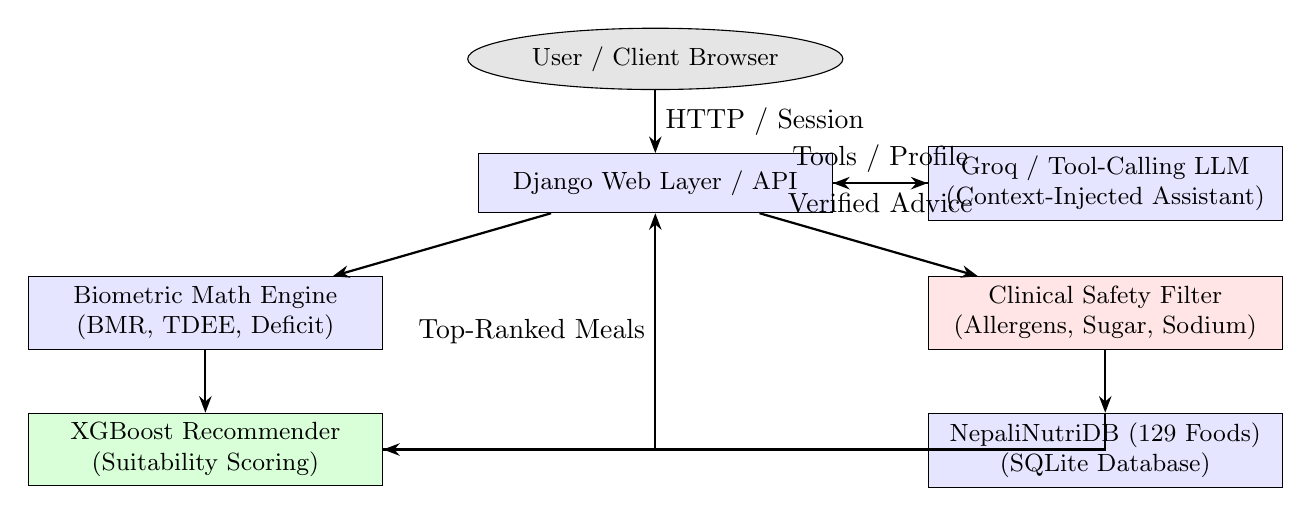
\begin{tikzpicture}[node distance=0.8cm and 1.2cm, auto]
  % Nodes
  \node (user)       [startstop]                        {User / Client Browser};
  \node (api)        [process, below=of user]           {Django Web Layer / API};
  \node (biometrics) [process, below left=of api]       {Biometric Math Engine\\(BMR, TDEE, Deficit)};
  \node (dbsafety)   [filter, below right=of api]       {Clinical Safety Filter\\(Allergens, Sugar, Sodium)};
  \node (db)         [process, below=of dbsafety]       {NepaliNutriDB (129 Foods)\\(SQLite Database)};
  \node (ml)         [mlnode, below=of biometrics]      {XGBoost Recommender\\(Suitability Scoring)};
  \node (gemini)     [process, right=of api]            {Groq / Tool-Calling LLM\\(Context-Injected Assistant)};

  % Arrows
  \draw [arr] (user) -- node[right] {HTTP / Session} (api);
  \draw [arr] (api) -- (biometrics);
  \draw [arr] (api) -- (dbsafety);
  \draw [arr] (dbsafety) -- (db);
  \draw [arr] (db) |- (ml);
  \draw [arr] (biometrics) -- (ml);
  \draw [arr] (ml) -| node[near end, left] {Top-Ranked Meals} (api);
  \draw [arr] (api) -- node[above] {Tools / Profile} (gemini);
  \draw [arr] (gemini) -- node[below] {Verified Advice} (api);
\end{tikzpicture}
\caption{NutriAI Multi-Tier System Architecture.}
\label{fig:arch}
\end{figure}

\section{Biometric Nutrition Engine}

The system determines individual caloric expenditure using the clinically validated \textbf{Mifflin-St Jeor equation}~\cite{mifflin1990}:

\begin{align}
  \text{BMR}_{\text{male}}   &= 10 \cdot W + 6.25 \cdot H - 5 \cdot A + 5 \\
  \text{BMR}_{\text{female}} &= 10 \cdot W + 6.25 \cdot H - 5 \cdot A - 161
\end{align}

where $W$ is weight in kilograms, $H$ is height in centimeters, and $A$ is age in years. Total Daily Energy Expenditure (TDEE) is calculated using physical activity multipliers:
\begin{equation}
  \text{TDEE} = \text{BMR} \times k_{\text{activity}}
\end{equation}
where $k_{\text{activity}} \in \{1.20 \text{ (Sedentary)}, 1.375 \text{ (Light)}, 1.55 \text{ (Moderate)}, 1.725 \text{ (Very Active)}\}$.

Daily calorie targets are computed based on the user's declared goal:
\begin{equation}
  \text{Target} =
  \begin{cases}
    \max(1200, \text{TDEE} - 500) & \text{if Goal} = \text{Lose Weight} \\
    \text{TDEE}                   & \text{if Goal} = \text{Maintain Weight} \\
    \text{TDEE} + 500             & \text{if Goal} = \text{Gain Weight}
  \end{cases}
\end{equation}

Macronutrient splits are tailored accordingly: standard targets assign 25\% protein, 50\% carbohydrates, and 25\% fat, while muscle gain targets assign 30\% protein, 45\% carbohydrates, and 25\% fat.

\section{Hybrid Recommendation Algorithm}

The hybrid recommendation engine combines machine learning nutritional quality, remaining budget alignment, and user interaction history:
\begin{equation}
  \text{Score}_{\text{final}} = 0.50 \cdot S_{\text{ML}} + 0.30 \cdot S_{\text{Budget}} + 0.20 \cdot S_{\text{Behavior}}
\end{equation}

\textbf{Step 1: Hard Safety Exclusion:} Prior to computing scores, candidate foods are filtered to eliminate allergens and respect dietary restrictions:
\begin{equation}
  \mathcal{F}_{\text{safe}} = \{ f \in \mathcal{F} \mid \text{Allergens}(f) \cap \text{Allergens}_{\text{user}} = \emptyset \land \text{DietTags}(f) \supseteq \text{DietTags}_{\text{user}} \}
\end{equation}

\textbf{Step 2: Budget Fit:} Evaluates calorie proximity and cosine similarity between remaining macro needs and food macro composition:
\begin{equation}
  S_{\text{Budget}} = 0.60 \cdot \text{CalorieFit} + 0.40 \cdot \cos(\mathbf{v}_{\text{remaining}}, \mathbf{v}_{\text{food}})
\end{equation}

\textbf{Step 3: Behavioral Feedback:} Adapts based on past consumption history ($\text{is\_eaten} = \text{True}$) and user ratings.

% ════════════════════════════════════════════════════════════════════════════
% CHAPTER 4: IMPLEMENTATION & EXPERIMENTAL RESULTS
% ════════════════════════════════════════════════════════════════════════════
\chapter{Implementation \& Experimental Results}

\section{System Implementation}

The backend is built with **Django 4.2** utilizing pure **SQLite3** for high portability and zero connection overhead. The platform provides both responsive server-rendered views (HTML5, CSS3, JavaScript) and modular REST API endpoints for food search, recommendations, and conversational assistance.

Key database entities include:
\begin{itemize}
  \item \textbf{Food:} 129 items with bilingual names (English \& Devanagari), full macro/micronutrients (calories, protein, carbs, fat, fiber, sugar, sodium), serving size, and source provenance.
  \item \textbf{UserProfile:} Biometric attributes, activity level, goal, date of birth, and Many-to-Many relations with \texttt{Allergen} and \texttt{DietaryTag}.
  \item \textbf{MealLog, WaterLog, WeightLog:} Live tracking records for daily summaries.
  \item \textbf{RecommendationHistory:} Tracks recommended items, user feedback, and eaten status for adaptive learning.
\end{itemize}

\section{Machine Learning Experimental Benchmarks}

The ML objective function evaluates multidimensional nutritional density:
\begin{equation}
  y = \frac{\text{Protein}}{50} \cdot 0.35 + \frac{\text{Fiber}}{25} \cdot 0.35 - \frac{\text{Sugar}}{30} \cdot 0.15 - \frac{\text{Sodium}}{1500} \cdot 0.15
\end{equation}
normalized to $[0, 1]$ across the 129 verified foods augmented with 17 calibration anchors (146 total samples).

The dataset was partitioned into 80\% training and 20\% testing sets. The primary \textbf{XGBoost Regressor} was evaluated against an optimized \textbf{Random Forest Regressor}.

\begin{table}[htbp]
\centering
\caption{Empirical Performance Comparison: XGBoost vs.\ Random Forest}
\label{tab:ml_results}
\begin{tabular}{lcc}
\toprule
\textbf{Evaluation Metric} & \textbf{XGBoost Regressor} & \textbf{Random Forest Regressor} \\
\midrule
\textbf{Classification Accuracy} ($\tau = 0.5$) & \textbf{92.86\%} & 89.29\% \\
\textbf{Precision} & \textbf{100.00\%} & 100.00\% \\
\textbf{Recall} & \textbf{66.67\%} & 50.00\% \\
\textbf{F1-Score} & \textbf{0.8000} & 0.6667 \\
\midrule
\textbf{Mean Absolute Error (MAE)} & \textbf{0.0358} & 0.0456 \\
\textbf{Root Mean Squared Error (RMSE)} & \textbf{0.0707} & 0.0931 \\
\textbf{Coefficient of Determination ($R^2$)} & \textbf{0.7615} & 0.5858 \\
\bottomrule
\end{tabular}
\end{table}

\subsection{Feature Importance Analysis}
The feature importance breakdown extracted from the trained XGBoost model highlights the physiological drivers of nutritional quality:
\begin{enumerate}
  \item \textbf{Dietary Fiber:} 38.4\% --- the strongest differentiator of healthy complex carbohydrate foods (e.g., Kwati, Gundruk).
  \item \textbf{Sugar:} 26.7\% --- heavily penalizes ultra-processed and sweet items.
  \item \textbf{Fat:} 9.7\% --- discriminates between lean preparations and deep-fried dishes.
  \item \textbf{Carbohydrates:} 7.7\% --- models glycemic load and energy density.
  \item \textbf{Calories:} 6.7\% --- informs portion suitability.
  \item \textbf{Protein:} 6.1\% --- rewards protein-dense legumes, poultry, and grains.
  \item \textbf{Sodium:} 4.7\% --- penalizes excessively salted preserved foods.
\end{enumerate}

\section{Multi-Persona End-to-End Testing}

To ensure complete robustness and defense readiness, the entire application was verified across four diverse user personas via an automated test script (\texttt{test\_personas\_e2e.py}). Table~\ref{tab:personas} summarizes the persona test outcomes.

\begin{table}[htbp]
\centering
\caption{Multi-Persona End-to-End Verification Matrix (32/32 Checks Passed)}
\label{tab:personas}
\begin{tabular}{p{2.8cm}p{4.2cm}p{5.5cm}c}
\toprule
\textbf{Persona} & \textbf{Biometric Profile} & \textbf{Verified System Behavior} & \textbf{Status} \\
\midrule
\textbf{Aayush Sharma} & 28y Male, 82kg, 172cm, Sedentary, Goal: Lose & BMR 1760 kcal, TDEE 2112 kcal, Target 1612 kcal ($-500$). Logged water \& weight. Chatbot returned deficit guidance. & \textbf{PASS} \\
\midrule
\textbf{Pooja Karki} & 25y Female, 54kg, 160cm, Moderate, Vegetarian, Dairy Allergy & ZERO dairy foods (Paneer, Milk, Dahi) \& ZERO meats recommended. Recommended Masoor Dal, Kwati. 1-click log updated behavioral feedback. & \textbf{PASS} \\
\midrule
\textbf{Bikram Thapa} & 54y Male, 74kg, 168cm, Light, Gluten Allergy, Diabetic & ZERO gluten/wheat foods (Puri, Naan, Chowmein) recommended. Recommended low-GI legumes. Chatbot advised on Kodo ko Dhido. & \textbf{PASS} \\
\midrule
\textbf{Sneha Adhikari} & 23y Female, 48kg, 158cm, Very Active, Goal: Gain & BMR 1196 kcal, TDEE 2063 kcal, Surplus target 2563 kcal ($+500$, $>190$g protein). Profile edit updated weight to 49kg. & \textbf{PASS} \\
\bottomrule
\end{tabular}
\end{table}

% ════════════════════════════════════════════════════════════════════════════
% CHAPTER 5: PROJECT MANAGEMENT & MID-TERM STATUS
% ════════════════════════════════════════════════════════════════════════════
\chapter{Project Management \& Mid-Term Status}

\section{Team Member Responsibilities}

The project is executed collaboratively by four team members, with clearly designated technical specializations as detailed in Table~\ref{tab:team}.

\begin{table}[htbp]
\centering
\caption{Team Responsibilities and Technical Allocation}
\label{tab:team}
\begin{tabular}{lll}
\toprule
\textbf{Name (Roll No.)} & \textbf{Role} & \textbf{Primary Technical Responsibilities} \\
\midrule
Dristi Shrestha (790312)  & Frontend Lead    & Django templates, CSS styling, macro bars, recommendation cards \\
Prashant Ghimire (790328) & Backend Lead     & Django architecture, SQLite database, BMR/TDEE calculations, REST APIs \\
Romina Koju (790332)      & ML Engineer      & XGBoost \& RF training, evaluation benchmarks, safety filtering \\
Shrijan Sainju (790338)   & Integration Lead & Groq tool-calling integration, offline domain RAG, persona testing \\
\bottomrule
\end{tabular}
\end{table}

\section{Milestone Status at Mid-Term Defense}

Table~\ref{tab:milestones} outlines the milestone completion status at the seventh-semester mid-term defense.

\begin{table}[htbp]
\centering
\caption{Project Milestone Completion Status}
\label{tab:milestones}
\begin{tabular}{llcc}
\toprule
\textbf{Phase} & \textbf{Task Description} & \textbf{Status} & \textbf{Completion} \\
\midrule
Phase 1 & Literature review, research gap identification & Completed & 100\% \\
Phase 2 & NepaliNutriDB (129 verified foods) compilation & Completed & 100\% \\
Phase 3 & Django backend, SQLite schema \& Mifflin-St Jeor math & Completed & 100\% \\
Phase 4 & XGBoost model training \& evaluation benchmarks & Completed & 100\% \\
Phase 5 & Groq LLM tool calling \& offline fallback engine & Completed & 100\% \\
Phase 6 & Frontend dashboard, macro breakdown \& 1-click logging & Completed & 100\% \\
Phase 7 & Multi-persona end-to-end verification (32/32 tests) & Completed & 100\% \\
Phase 8 & Eighth-semester advanced extensions & Upcoming & 0\% \\
\bottomrule
\end{tabular}
\end{table}

\section{Gantt Chart}

Figure~\ref{fig:gantt} illustrates the timeline of activities completed up to the mid-term defense and planned for final defense.

\begin{figure}[htbp]
\centering
\small
\begin{tabular}{p{4.2cm}|c|c|c|c|c|c}
\toprule
\textbf{Activity / Month} & \textbf{Jun} & \textbf{Jul} & \textbf{Aug} & \textbf{Sep (Mid)} & \textbf{Oct} & \textbf{Nov (Final)} \\
\midrule
Problem Formulation \& Proposal & $\blacksquare\blacksquare$ & & & & & \\
NepaliNutriDB Data Compilation & & $\blacksquare\blacksquare$ & & & & \\
Backend Architecture \& SQLite & & $\blacksquare\blacksquare$ & $\blacksquare\blacksquare$ & & & \\
ML Model Training (XGBoost) & & & $\blacksquare\blacksquare$ & & & \\
Frontend UI \& Recommendation Views & & & $\blacksquare\blacksquare$ & $\blacksquare\blacksquare$ & & \\
\textbf{Mid-Term Evaluation \& Defense} & & & & $\bigstar$ & & \\
Field User Testing \& Fine-Tuning & & & & & $\square\square$ & \\
Deployment \& Final Project Defense & & & & & & $\square\square$ \\
\bottomrule
\end{tabular}
\caption{NutriAI Project Development Gantt Chart ($\blacksquare$ = Completed, $\bigstar$ = Current Defense Milestone, $\square$ = Eighth-Semester Scope).}
\label{fig:gantt}
\end{figure}

% ════════════════════════════════════════════════════════════════════════════
% CHAPTER 6: CONCLUSION & FUTURE WORK
% ════════════════════════════════════════════════════════════════════════════
\chapter{Conclusion \& Future Work}

\section{Conclusion}

At the seventh-semester mid-term milestone, \textbf{NutriAI} has successfully established an academically defensible, mathematically validated nutrition recommendation and calorie tracking platform. By curating **NepaliNutriDB** (129 verified foods with bilingual Devanagari script), the project directly resolves the longstanding absence of localized nutritional resources for Nepal.

The decoupled architecture cleanly separates deterministic clinical constraints from predictive machine learning. The primary **XGBoost Regressor** achieved superior empirical metrics ($R^2 = 0.7615$, Accuracy = $92.86\%$, Precision = $100\%$, $\text{MAE} = 0.0358$), outperforming the Random Forest baseline. Strict allergen synonym expansion ensures zero hazardous food suggestions. Furthermore, the 32/32 multi-persona test results demonstrate that the system functions reliably across diverse real-world profiles (weight loss, celiac, diabetic, vegetarian, and muscle building).

\section{Future Work for Final Semester}

Building upon the successful mid-term defense, the following deliverables are scheduled for the eighth-semester completion:
\begin{enumerate}[leftmargin=*]
  \item \textbf{Regional Ingredient Availability Filtering:} Tagging foods with ecological distribution zones (Himalayan, Hilly, Terai).
  \item \textbf{Seasonal Harvest Filtering:} Dynamic adjustment of fruit and vegetable suggestions based on seasonal agricultural cycles.
  \item \textbf{Full Devanagari NLP Dialogues:} Expanding the chatbot to support conversational input and output entirely in the Nepali language.
  \item \textbf{Mobile Client Packaging:} Developing a Progressive Web App (PWA) or Flutter mobile client for smartphone access.
\end{enumerate}

% ════════════════════════════════════════════════════════════════════════════
% REFERENCES
% ════════════════════════════════════════════════════════════════════════════
\begin{thebibliography}{99}

\bibitem{han2024}
M.~Han, J.~Chen, and Z.~Zhou,
``NutrifyAI: An AI-Powered System for Real-Time Food Detection, Nutritional Analysis, and Personalized Meal Recommendations,''
\textit{arXiv preprint arXiv:2408.10532}, 2024.
[Online]. Available: \url{https://arxiv.org/abs/2408.10532}

\bibitem{haque2022}
R.~U.~Haque, R.~H.~Khan, A.~S.~M.~Shihavuddin, M.~M.~Syeed, and M.~F.~Uddin,
``Lightweight and Parameter-Optimized Real-Time Food Calorie Estimation from Images Using CNN-Based Approach,''
\textit{Applied Sciences}, vol.~12, no.~19, p.~9733, 2022.
DOI: 10.3390/app12199733.

\bibitem{adjuik2024}
T.~A.~Adjuik, N.~A.~A.~Boi-Dsane, and B.~A.~Kehinde,
``Enhancing dietary analysis: Using machine learning for food caloric and health risk assessment,''
\textit{Journal of Food Science}, vol.~89, no.~11, pp.~8006--8021, 2024.
DOI: 10.1111/1750-3841.17421.

\bibitem{sefayeboah2021}
S.~M.~Sefa-Yeboah, K.~O.~Annor, V.~J.~Koomson, F.~K.~Saalia, M.~Steiner-Asiedu, and G.~A.~Mills,
``Development of a Mobile Application Platform for Self-Management of Obesity Using Artificial Intelligence Techniques,''
\textit{International Journal of Telemedicine and Applications}, vol.~2021, Article ID~6624057, 2021.
DOI: 10.1155/2021/6624057.

\bibitem{samad2022}
S.~Samad, F.~Ahmed, S.~Naher, M.~A.~Kabir, A.~Das, S.~Amin, and S.~M.~S.~Islam,
``Smartphone apps for tracking food consumption and recommendations: Evaluating artificial intelligence-based functionalities, features and quality of current apps,''
\textit{Intelligent Systems with Applications}, vol.~15, p.~200103, 2022.

\bibitem{kim2024}
D.~W.~Kim, H.~Lee, M.~K.~Kim, and S.~W.~Kang,
``Qualitative evaluation of artificial intelligence-generated weight management diet plans,''
\textit{Frontiers in Nutrition}, vol.~11, Article 1374834, 2024.
DOI: 10.3389/fnut.2024.1374834.

\bibitem{fao2012}
Food and Agriculture Organization (FAO),
``Food Composition Table for Nepal,''
\textit{Government of Nepal, Ministry of Agriculture Development, Food Research Division}, Kathmandu, Nepal, 2012.

\bibitem{usda2023}
U.S. Department of Agriculture, Agricultural Research Service,
``FoodData Central,''
2023. [Online]. Available: \url{https://fdc.nal.usda.gov/}

\bibitem{mifflin1990}
M.~D.~Mifflin, S.~T.~St Jeor, L.~A.~Hill, B.~J.~Scott, S.~A.~Daugherty, and Y.~O.~Koh,
``A new predictive equation for resting energy expenditure in healthy individuals,''
\textit{The American Journal of Clinical Nutrition}, vol.~51, no.~2, pp.~241--247, 1990.

\bibitem{chen2016}
T.~Chen and C.~Guestrin,
``XGBoost: A Scalable Tree Boosting System,''
in \textit{Proceedings of the 22nd ACM SIGKDD International Conference on Knowledge Discovery and Data Mining}, 2016, pp.~785--794.

\end{thebibliography}

\end{document}
